\documentclass[12pt]{article}

\usepackage[utf8]{inputenc}
\usepackage{geometry}
\usepackage{listings}
\geometry{a4paper, margin=1in}
\usepackage{graphicx}
\usepackage{hyperref}
\usepackage{fancyhdr}

\pagestyle{fancy}
\fancyhead[L]{\thepage}
\fancyfoot[C]{\texttt{HW-402521189} }

\begin{document}
\title{Computer Workshop\\Final Assignment} 
\date{ 7,Bahman,1402 } %mishof \today zad vali hkob miladi gharar midad
\author{\\ Dr. MalekiMajd \\ \\ \\ \emph{Creator :}\\ \emph{\texttt{Matin Hasanali Baki }}  \\ \\ \underline{SID :    402521189} \\ \\ \\  }
\maketitle

\newpage
\begin{quote}
\end{quote}
\tableofcontents

\newpage




\section*{Information}
links and ...


\section{Git and GitHub}
\subsection{Repository Initialization and Commits}


\subsection{GitHub Actions for LaTeX Compilation}



\section{Exploration Tasks}
\subsection{Vim Advanced Features}
\begin{itemize}
  \item ctrl+n   or  ctrl+p\newline With its help, you can auto complete, for example, the following text:\newline Matin Modem Salam Saeed Return,By typing {M} and then pressing the above command, you can select one of the typed words that starts with this structure, that is, in this example:\newline
  Matin/Modem\newline
  With its help, you can auto complete, for example, the following text:\newline
Matin Modem Salam Saeed Return
By typing {M} and then pressing the above command, you can select one of the typed words that starts with this structure, that is, in this example:
Matin/Modem
  \item gf/gx
      \begin{itemize}
        \item gf
        With its help, you can use the address of a typed directory and create a new buffer file.\newline
        C://Users/Desktop/matin.txt + {gf}
        \item gx
        With its help, you can open a typed website address\newline
        https://quera.org/course/15588/ + {gx}
      \end{itemize}



  \item :X\newline
  With its help, a file can be encrypted and its content cannot be viewed outside Vim, for example, with the help of content extraction commands, or even
  To open that file, you must enter the password that has been set\newline
  :X    ----   Enter encryption key : ****   ----  Enter same encryption key again : ****
\end{itemize}

\subsection{Memory profiling}
\subsubsection{Memory Leak}

This definition occurs when the programmer allocates a memory but does not use it (for any reason, such as forgetfulness, mistakes, incompleteness, or even laziness) and obviously This memory will be involved until it disappears, and the point is that we may no longer need what we allocated, and this means reducing the amount of available memory while running the program.And that means slowing down the execution of the program or even exiting the execution of the program (yes)
\newpage
 reasons :
\begin{itemize}
  \item Not calling for free
  \item Jumping (losing) the address where you allocated memory (and this means that even if we want to delete, we don't know where we saved the memory to delete it, example code:)\newline
  \begin{lstlisting}
  int *ptr=(int * )malloc(sizeof(int)) ;
  int x=5 ;
  ptr=&x ;
  free(????) ;
  \end{lstlisting}
  \item We do not put the conditioning of the fairy and it in the general state (for example:)\newline
  \begin{lstlisting}
    int *ptr=(int * )malloc(sinzeof(int)) ;
    int x ;
    scanf("%d",&x) ;
    if(x%2==0){printf("E") ; free(ptr) ;}
    if(x%2==1){printf("O") ; }
  \end{lstlisting}
  \item If you exit or exit the program while the program is running and the Fairy part has not yet run, it is possible that the memory will not be freed and it will produce a story in the next run and it will become unstable.


\end{itemize}

\subsubsection{Memory profilers}
A tool that can be used to show the memory error that is due to access to the heap memory, the type of error and the location of the error in the C or C++ code.
And it helps in finding the bug codes in this type of error, which means saving time and effort...\newline
And this program can be run in Linux!\newline
It clarifies the errors for us and with its help we can fix these errors more easily
\texttt{ memory leaks, reading uninitialized memory, accessing unallocated memory, and array out-of-bounds}
.And with the help of the information that the program gives us, a code error occurs (or at least we understand that we have a memory problem).
\begin{lstlisting}
heap:
? allocs, ? free bytes allocated
leaks:
? bytes in ? blocks
And...
\end{lstlisting}
This information can be found in the leak section especially if there is a problem or not.

\newpage
\subsection{GNU/Linux Bash Scripting}


\subsubsection{fzf}
\begin{itemize}
  \item What is fuzzy searching?\newline
  It is a search algorithm, the purpose of this algorithm is if we are looking for an article and we know only one article that includes that discussion.
Or even if we only know the name of the topic or know anything related to it, this operation will be executed at the time of searching with the help of this algorithm.
The good thing about this algorithm is that it ranks based on the number of matches of our search with the database it has and lists and displays them in order of priority.
And he can even tell if this is what you meant according to the database he has, that is, he can correct it if there is a mistake.
\item what the following command does: \texttt{ls | fzf}\newline
It pins the list of directories created by \texttt{ls} and produces a mode, one can select the desired directory by scrolling up and down and enter it.
\end{itemize}



\subsubsection{Using fzf to find your favorite PDF}
\texttt{fd -e pdf \{finds all files of this type\}}\newline
\texttt{fzf --query="???" \{all files whose name has "???"\}}\newline
So, after piping, we will have a series of PDF files named \texttt{???} They are in themselves\newline
\texttt{fd-e pdf | fzf --query="???"}


\subsubsection{Opening the file using Zathura}
\texttt{zathura "\$(fd -e pdf | fzf --query="???")"} \newline
As mentioned, the command written in parentheses opens a list to select the desired file and we select it by up and down, but actually we enter that directory and the PDF file does not open.
To open it, we can use the above command, and in fact, it will open the PDF file in the directory we give it.
\newline
In a way, it can be said that we hit another pipe...
\newline
\texttt{zathura PATH\_PDF or zathura NAMEPDF.pdf}

\section{Git and FOSS}

\subsubsection{README.md}
\begin{figure}

  \centering

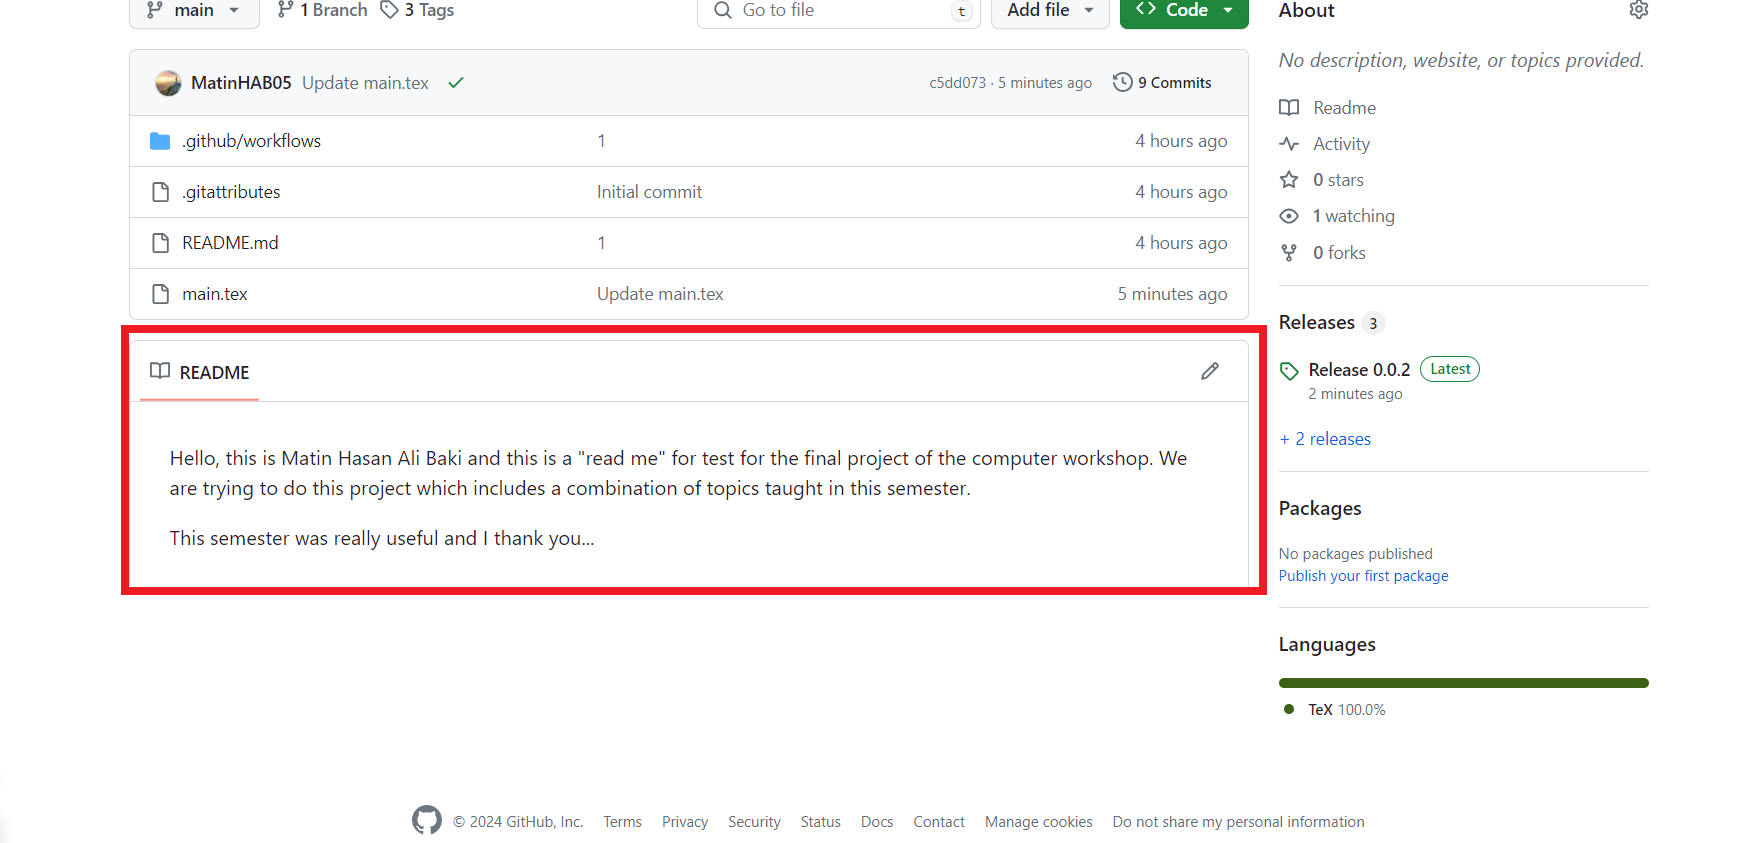
\includegraphics[width=0.8\textwidth]{read.png}

\caption{Done!}


\end{figure}

\subsection{Issues}
\begin{figure}

  \centering

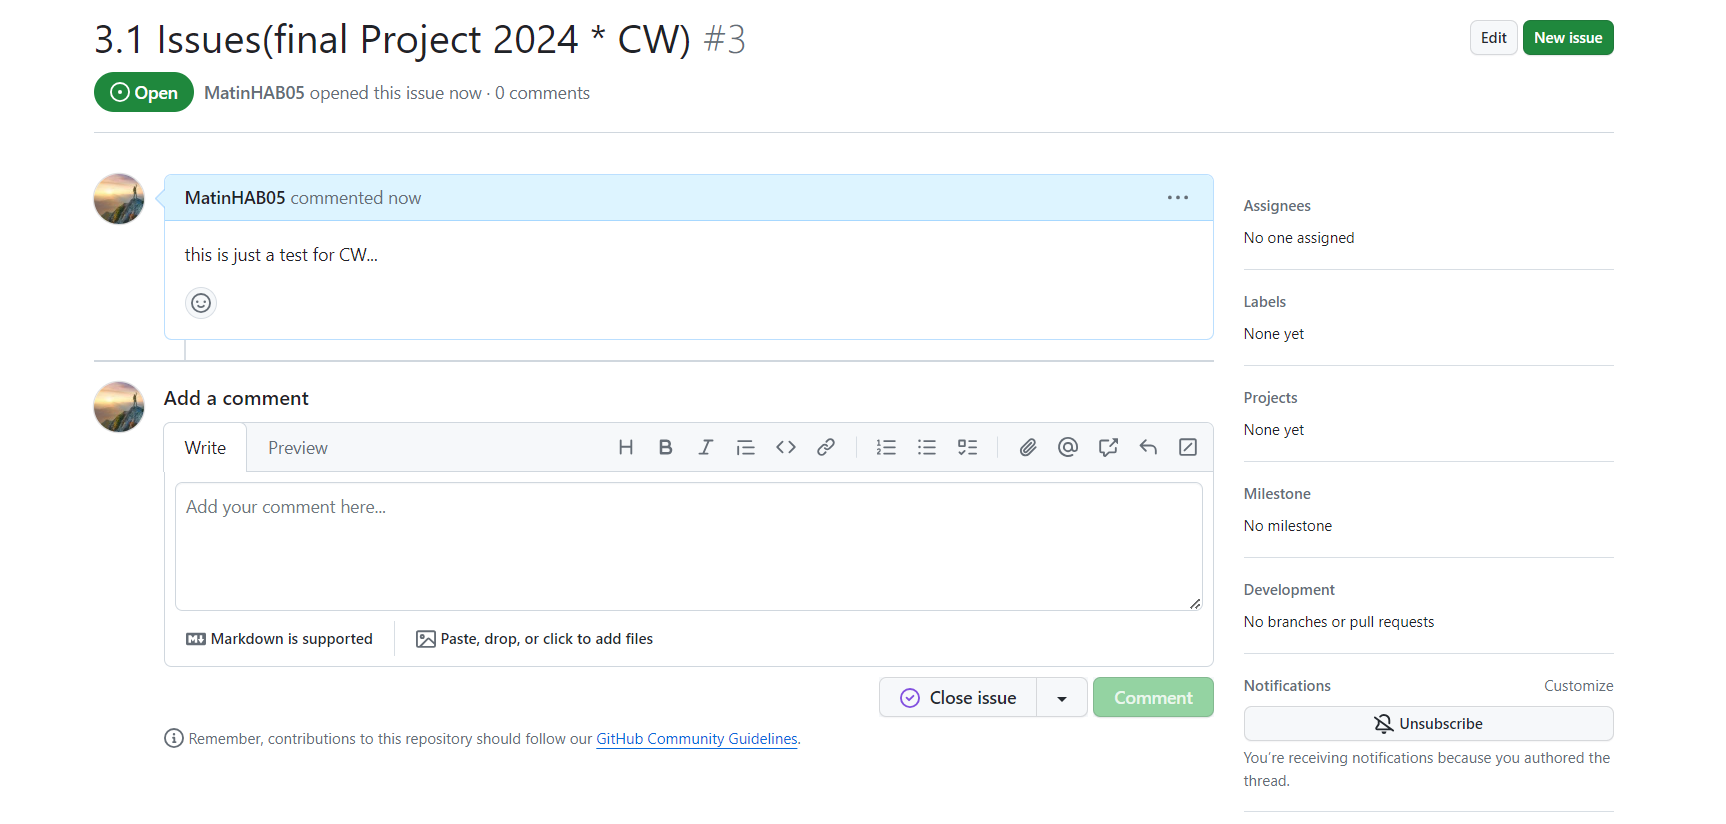
\includegraphics[width=0.8\textwidth]{is.png}

\caption{Done!}


\end{figure}

\end{document}
